% Options for packages loaded elsewhere
\PassOptionsToPackage{unicode}{hyperref}
\PassOptionsToPackage{hyphens}{url}
\PassOptionsToPackage{dvipsnames,svgnames,x11names}{xcolor}
\documentclass[
  11pt,
]{article}
\usepackage{xcolor}
\usepackage[margin=0.5in]{geometry}
\usepackage{amsmath,amssymb}
\setcounter{secnumdepth}{5}
\usepackage{iftex}
\ifPDFTeX
  \usepackage[T1]{fontenc}
  \usepackage[utf8]{inputenc}
  \usepackage{textcomp} % provide euro and other symbols
\else % if luatex or xetex
  \usepackage{unicode-math} % this also loads fontspec
  \defaultfontfeatures{Scale=MatchLowercase}
  \defaultfontfeatures[\rmfamily]{Ligatures=TeX,Scale=1}
\fi
\usepackage{lmodern}
\ifPDFTeX\else
  % xetex/luatex font selection
  \setmainfont[]{Helvetica}
  \setmonofont[]{Menlo}
\fi
% Use upquote if available, for straight quotes in verbatim environments
\IfFileExists{upquote.sty}{\usepackage{upquote}}{}
\IfFileExists{microtype.sty}{% use microtype if available
  \usepackage[]{microtype}
  \UseMicrotypeSet[protrusion]{basicmath} % disable protrusion for tt fonts
}{}
\makeatletter
\@ifundefined{KOMAClassName}{% if non-KOMA class
  \IfFileExists{parskip.sty}{%
    \usepackage{parskip}
  }{% else
    \setlength{\parindent}{0pt}
    \setlength{\parskip}{6pt plus 2pt minus 1pt}}
}{% if KOMA class
  \KOMAoptions{parskip=half}}
\makeatother
\usepackage{color}
\usepackage{fancyvrb}
\newcommand{\VerbBar}{|}
\newcommand{\VERB}{\Verb[commandchars=\\\{\}]}
\DefineVerbatimEnvironment{Highlighting}{Verbatim}{commandchars=\\\{\}}
% Add ',fontsize=\small' for more characters per line
\usepackage{framed}
\definecolor{shadecolor}{RGB}{248,248,248}
\newenvironment{Shaded}{\begin{snugshade}}{\end{snugshade}}
\newcommand{\AlertTok}[1]{\textcolor[rgb]{0.94,0.16,0.16}{#1}}
\newcommand{\AnnotationTok}[1]{\textcolor[rgb]{0.56,0.35,0.01}{\textbf{\textit{#1}}}}
\newcommand{\AttributeTok}[1]{\textcolor[rgb]{0.13,0.29,0.53}{#1}}
\newcommand{\BaseNTok}[1]{\textcolor[rgb]{0.00,0.00,0.81}{#1}}
\newcommand{\BuiltInTok}[1]{#1}
\newcommand{\CharTok}[1]{\textcolor[rgb]{0.31,0.60,0.02}{#1}}
\newcommand{\CommentTok}[1]{\textcolor[rgb]{0.56,0.35,0.01}{\textit{#1}}}
\newcommand{\CommentVarTok}[1]{\textcolor[rgb]{0.56,0.35,0.01}{\textbf{\textit{#1}}}}
\newcommand{\ConstantTok}[1]{\textcolor[rgb]{0.56,0.35,0.01}{#1}}
\newcommand{\ControlFlowTok}[1]{\textcolor[rgb]{0.13,0.29,0.53}{\textbf{#1}}}
\newcommand{\DataTypeTok}[1]{\textcolor[rgb]{0.13,0.29,0.53}{#1}}
\newcommand{\DecValTok}[1]{\textcolor[rgb]{0.00,0.00,0.81}{#1}}
\newcommand{\DocumentationTok}[1]{\textcolor[rgb]{0.56,0.35,0.01}{\textbf{\textit{#1}}}}
\newcommand{\ErrorTok}[1]{\textcolor[rgb]{0.64,0.00,0.00}{\textbf{#1}}}
\newcommand{\ExtensionTok}[1]{#1}
\newcommand{\FloatTok}[1]{\textcolor[rgb]{0.00,0.00,0.81}{#1}}
\newcommand{\FunctionTok}[1]{\textcolor[rgb]{0.13,0.29,0.53}{\textbf{#1}}}
\newcommand{\ImportTok}[1]{#1}
\newcommand{\InformationTok}[1]{\textcolor[rgb]{0.56,0.35,0.01}{\textbf{\textit{#1}}}}
\newcommand{\KeywordTok}[1]{\textcolor[rgb]{0.13,0.29,0.53}{\textbf{#1}}}
\newcommand{\NormalTok}[1]{#1}
\newcommand{\OperatorTok}[1]{\textcolor[rgb]{0.81,0.36,0.00}{\textbf{#1}}}
\newcommand{\OtherTok}[1]{\textcolor[rgb]{0.56,0.35,0.01}{#1}}
\newcommand{\PreprocessorTok}[1]{\textcolor[rgb]{0.56,0.35,0.01}{\textit{#1}}}
\newcommand{\RegionMarkerTok}[1]{#1}
\newcommand{\SpecialCharTok}[1]{\textcolor[rgb]{0.81,0.36,0.00}{\textbf{#1}}}
\newcommand{\SpecialStringTok}[1]{\textcolor[rgb]{0.31,0.60,0.02}{#1}}
\newcommand{\StringTok}[1]{\textcolor[rgb]{0.31,0.60,0.02}{#1}}
\newcommand{\VariableTok}[1]{\textcolor[rgb]{0.00,0.00,0.00}{#1}}
\newcommand{\VerbatimStringTok}[1]{\textcolor[rgb]{0.31,0.60,0.02}{#1}}
\newcommand{\WarningTok}[1]{\textcolor[rgb]{0.56,0.35,0.01}{\textbf{\textit{#1}}}}
\usepackage{longtable,booktabs,array}
\newcounter{none} % for unnumbered tables
\usepackage{calc} % for calculating minipage widths
% Correct order of tables after \paragraph or \subparagraph
\usepackage{etoolbox}
\makeatletter
\patchcmd\longtable{\par}{\if@noskipsec\mbox{}\fi\par}{}{}
\makeatother
% Allow footnotes in longtable head/foot
\IfFileExists{footnotehyper.sty}{\usepackage{footnotehyper}}{\usepackage{footnote}}
\makesavenoteenv{longtable}
\usepackage{graphicx}
\makeatletter
\newsavebox\pandoc@box
\newcommand*\pandocbounded[1]{% scales image to fit in text height/width
  \sbox\pandoc@box{#1}%
  \Gscale@div\@tempa{\textheight}{\dimexpr\ht\pandoc@box+\dp\pandoc@box\relax}%
  \Gscale@div\@tempb{\linewidth}{\wd\pandoc@box}%
  \ifdim\@tempb\p@<\@tempa\p@\let\@tempa\@tempb\fi% select the smaller of both
  \ifdim\@tempa\p@<\p@\scalebox{\@tempa}{\usebox\pandoc@box}%
  \else\usebox{\pandoc@box}%
  \fi%
}
% Set default figure placement to htbp
\def\fps@figure{htbp}
\makeatother
\setlength{\emergencystretch}{3em} % prevent overfull lines
\providecommand{\tightlist}{%
  \setlength{\itemsep}{0pt}\setlength{\parskip}{0pt}}
\usepackage{xcolor}
\usepackage{fvextra}
\DefineVerbatimEnvironment{Highlighting}{Verbatim}{breaklines,breakanywhere,commandchars=\\\{\}}
\usepackage{graphicx}
\usepackage{float}
\usepackage{microtype}
\usepackage{setspace}
\usepackage{bookmark}
\IfFileExists{xurl.sty}{\usepackage{xurl}}{} % add URL line breaks if available
\urlstyle{same}
\hypersetup{
  pdftitle={Urban Tree Methods with the USDA Urban Tree Database},
  pdfauthor={Rebecca Bronstein},
  colorlinks=true,
  linkcolor={blue},
  filecolor={Maroon},
  citecolor={Blue},
  urlcolor={blue},
  pdfcreator={LaTeX via pandoc}}

\title{Urban Tree Methods with the USDA Urban Tree Database}
\author{Rebecca Bronstein}
\date{2026-04-01}

\begin{document}
\maketitle

{
\setcounter{tocdepth}{2}
\tableofcontents
}
\subsection{Data Source}\label{data-source}

This report uses the USDA Forest Service Research Data Archive
publication \textbf{Urban tree database} and the local file
\texttt{Data/TS3\_Raw\_tree\_data.csv} included in this folder. The
archive describes the publication as a multi-city urban tree dataset
covering more than 14,000 measured urban trees across 17 U.S. cities.
Source page:
\url{https://www.fs.usda.gov/rds/archive/catalog/RDS-2016-0005}.

\subsection{Why Tree Methods Fit This
Dataset}\label{why-tree-methods-fit-this-dataset}

This archive mixes species, urban form, and tree structure in the same
table. Tree methods are a natural fit because they can move between
those data types without flattening the whole problem into one linear
rule.

I use tree methods here to answer four practical questions:

\begin{enumerate}
\def\labelenumi{\arabic{enumi}.}
\tightlist
\item
  Can a tree's structure and site context tell us whether it came from a
  street setting or a more park-like one?
\item
  Which measurements matter most when predicting height?
\item
  Can a short rule set explain which trees produce stronger car shade?
\item
  How do different classification methods trade speed for accuracy when
  the target is much harder, such as \texttt{TreeType}?
\end{enumerate}

\subsection{Data Snapshot}\label{data-snapshot}

\begin{Shaded}
\begin{Highlighting}[]
\FunctionTok{kable}\NormalTok{(overview, }\AttributeTok{caption =} \StringTok{"USDA urban tree data summary."}\NormalTok{)}
\end{Highlighting}
\end{Shaded}

\begin{longtable}[]{@{}lr@{}}
\caption{USDA urban tree data summary.}\tabularnewline
\toprule\noalign{}
Measure & Value \\
\midrule\noalign{}
\endfirsthead
\toprule\noalign{}
Measure & Value \\
\midrule\noalign{}
\endhead
\bottomrule\noalign{}
\endlastfoot
Total tree records & 14487 \\
Distinct cities & 17 \\
Distinct climate regions & 17 \\
Street trees & 8987 \\
Park-like trees & 5500 \\
Distinct tree types & 12 \\
\end{longtable}

\subsection{Visual Briefing}\label{visual-briefing}

The two figures below keep the ink budget low and let the data do most
of the talking. The first shows how strongly the share of street trees
varies by region. The second shows a familiar forestry relationship:
height rises with diameter, but the slope and spread differ across site
types.

\begin{Shaded}
\begin{Highlighting}[]
\FunctionTok{ggplot}\NormalTok{(site\_mix, }\FunctionTok{aes}\NormalTok{(}\AttributeTok{x =}\NormalTok{ Share, }\AttributeTok{y =} \FunctionTok{fct\_reorder}\NormalTok{(Region, Share))) }\SpecialCharTok{+}
  \FunctionTok{geom\_segment}\NormalTok{(}\FunctionTok{aes}\NormalTok{(}\AttributeTok{x =} \DecValTok{0}\NormalTok{, }\AttributeTok{xend =}\NormalTok{ Share, }\AttributeTok{yend =}\NormalTok{ Region), }\AttributeTok{color =} \StringTok{"grey82"}\NormalTok{, }\AttributeTok{linewidth =} \FloatTok{0.35}\NormalTok{) }\SpecialCharTok{+}
  \FunctionTok{geom\_point}\NormalTok{(}\AttributeTok{size =} \FloatTok{1.8}\NormalTok{, }\AttributeTok{color =} \StringTok{"black"}\NormalTok{) }\SpecialCharTok{+}
  \FunctionTok{scale\_x\_continuous}\NormalTok{(}\AttributeTok{labels =}\NormalTok{ scales}\SpecialCharTok{::}\FunctionTok{percent\_format}\NormalTok{(}\AttributeTok{accuracy =} \DecValTok{1}\NormalTok{)) }\SpecialCharTok{+}
  \FunctionTok{labs}\NormalTok{(}
    \AttributeTok{title =} \StringTok{"Street share varies sharply across climate regions"}\NormalTok{,}
    \AttributeTok{subtitle =} \StringTok{"Each point is the share of observations classified as street trees within a region"}\NormalTok{,}
    \AttributeTok{x =} \StringTok{"Street share"}\NormalTok{,}
    \AttributeTok{y =} \ConstantTok{NULL}
\NormalTok{  ) }\SpecialCharTok{+}
  \FunctionTok{theme\_lowink}\NormalTok{()}
\end{Highlighting}
\end{Shaded}

\pandocbounded{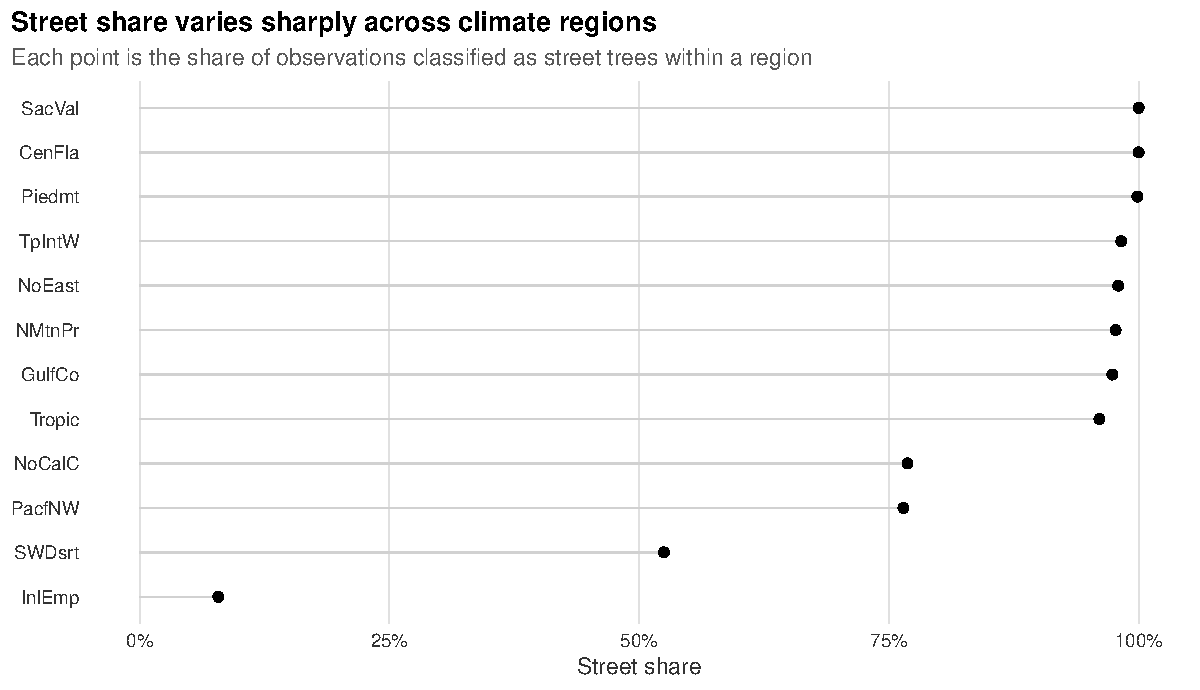
\includegraphics[keepaspectratio]{tree_tree_analysis_files/figure-latex/site_mix_plot-1.pdf}}

\begin{Shaded}
\begin{Highlighting}[]
\FunctionTok{ggplot}\NormalTok{(height\_profile, }\FunctionTok{aes}\NormalTok{(}\AttributeTok{x =}\NormalTok{ DBH, }\AttributeTok{y =}\NormalTok{ TreeHt, }\AttributeTok{color =}\NormalTok{ Site.Type)) }\SpecialCharTok{+}
  \FunctionTok{geom\_point}\NormalTok{(}\AttributeTok{alpha =} \FloatTok{0.18}\NormalTok{, }\AttributeTok{size =} \FloatTok{0.7}\NormalTok{, }\AttributeTok{stroke =} \DecValTok{0}\NormalTok{) }\SpecialCharTok{+}
  \FunctionTok{geom\_smooth}\NormalTok{(}\AttributeTok{method =} \StringTok{"loess"}\NormalTok{, }\AttributeTok{se =} \ConstantTok{FALSE}\NormalTok{, }\AttributeTok{linewidth =} \FloatTok{0.7}\NormalTok{) }\SpecialCharTok{+}
  \FunctionTok{scale\_color\_manual}\NormalTok{(}\AttributeTok{values =} \FunctionTok{c}\NormalTok{(}\StringTok{"Street"} \OtherTok{=} \StringTok{"grey20"}\NormalTok{, }\StringTok{"Park{-}like"} \OtherTok{=} \StringTok{"grey60"}\NormalTok{)) }\SpecialCharTok{+}
  \FunctionTok{labs}\NormalTok{(}
    \AttributeTok{title =} \StringTok{"Height rises with diameter, but not identically across site types"}\NormalTok{,}
    \AttributeTok{subtitle =} \StringTok{"A thin smoother carries the structure while the points preserve the raw spread"}\NormalTok{,}
    \AttributeTok{x =} \StringTok{"DBH (cm)"}\NormalTok{,}
    \AttributeTok{y =} \StringTok{"Tree height (m)"}
\NormalTok{  ) }\SpecialCharTok{+}
  \FunctionTok{theme\_lowink}\NormalTok{() }\SpecialCharTok{+}
  \FunctionTok{theme}\NormalTok{(}\AttributeTok{legend.position =} \FunctionTok{c}\NormalTok{(}\FloatTok{0.84}\NormalTok{, }\FloatTok{0.2}\NormalTok{))}
\end{Highlighting}
\end{Shaded}

\pandocbounded{
\includegraphics[keepaspectratio]{tree_tree_analysis_files/figure-latex/height_profile_plot-1.pdf}}

\subsection{Classification Tree: Street Trees vs.~Park-Like
Trees}\label{classification-tree-street-trees-vs.-park-like-trees}

The original \texttt{Park/Street} field includes a few tiny categories
such as nursery and regional big tree. For the main site-context model I
collapse those into a simpler binary outcome:

\begin{enumerate}
\def\labelenumi{\arabic{enumi}.}
\tightlist
\item
  \texttt{Street}
\item
  \texttt{Park-like}
\end{enumerate}

That turns the tree into a site classifier rather than a bookkeeping
exercise.

\begin{Shaded}
\begin{Highlighting}[]
\NormalTok{site\_tree }\OtherTok{\textless{}{-}} \FunctionTok{rpart}\NormalTok{(Site.Type }\SpecialCharTok{\textasciitilde{}}\NormalTok{ ., }\AttributeTok{data =}\NormalTok{ train\_site, }\AttributeTok{method =} \StringTok{"class"}\NormalTok{)}
\FunctionTok{plot}\NormalTok{(site\_tree, }\AttributeTok{uniform =} \ConstantTok{TRUE}\NormalTok{, }\AttributeTok{margin =} \FloatTok{0.08}\NormalTok{)}
\FunctionTok{text}\NormalTok{(site\_tree, }\AttributeTok{use.n =} \ConstantTok{TRUE}\NormalTok{, }\AttributeTok{cex =} \FloatTok{0.68}\NormalTok{)}
\end{Highlighting}
\end{Shaded}

\pandocbounded{
\includegraphics[keepaspectratio]{tree_tree_analysis_files/figure-latex/classification_tree-1.pdf}}

\begin{Shaded}
\begin{Highlighting}[]
\NormalTok{site\_pred }\OtherTok{\textless{}{-}} \FunctionTok{predict}\NormalTok{(site\_tree, test\_site, }\AttributeTok{type =} \StringTok{"class"}\NormalTok{)}
\NormalTok{site\_metrics }\OtherTok{\textless{}{-}} \FunctionTok{classification\_metrics}\NormalTok{(test\_site}\SpecialCharTok{$}\NormalTok{Site.Type, site\_pred)}
\NormalTok{site\_importance }\OtherTok{\textless{}{-}} \FunctionTok{top\_importance}\NormalTok{(site\_tree)}

\FunctionTok{kable}\NormalTok{(site\_metrics, }\AttributeTok{caption =} \StringTok{"Site{-}type classification performance."}\NormalTok{)}
\end{Highlighting}
\end{Shaded}

\begin{longtable}[]{@{}rr@{}}
\caption{Site-type classification performance.}\tabularnewline
\toprule\noalign{}
Accuracy & Kappa \\
\midrule\noalign{}
\endfirsthead
\toprule\noalign{}
Accuracy & Kappa \\
\midrule\noalign{}
\endhead
\bottomrule\noalign{}
\endlastfoot
0.989 & 0.975 \\
\end{longtable}

\begin{Shaded}
\begin{Highlighting}[]
\FunctionTok{kable}\NormalTok{(site\_importance, }\AttributeTok{caption =} \StringTok{"Top variables in the site{-}type tree."}\NormalTok{)}
\end{Highlighting}
\end{Shaded}

\begin{longtable}[]{@{}lr@{}}
\caption{Top variables in the site-type tree.}\tabularnewline
\toprule\noalign{}
Variable & Importance \\
\midrule\noalign{}
\endfirsthead
\toprule\noalign{}
Variable & Importance \\
\midrule\noalign{}
\endhead
\bottomrule\noalign{}
\endlastfoot
Region & 1203.50 \\
LandUse & 611.93 \\
TreeType & 47.93 \\
Age & 35.85 \\
Setback & 35.15 \\
Leaf & 30.09 \\
\end{longtable}

This model performs well because it is solving a strong structural
problem. Region, land use, and setback do most of the work, which is
exactly what we would expect if site design and management shape the
kinds of trees we observe.

\subsection{Regression Tree: What Predicts Tree
Height?}\label{regression-tree-what-predicts-tree-height}

Urban tree height sits at the center of many planning questions, but it
is not controlled by diameter alone. A regression tree lets the data
split into crown-based neighborhoods that are easier to interpret than
one global regression line.

\begin{Shaded}
\begin{Highlighting}[]
\NormalTok{height\_tree }\OtherTok{\textless{}{-}} \FunctionTok{rpart}\NormalTok{(TreeHt }\SpecialCharTok{\textasciitilde{}}\NormalTok{ ., }\AttributeTok{data =}\NormalTok{ train\_height, }\AttributeTok{method =} \StringTok{"anova"}\NormalTok{)}
\FunctionTok{plot}\NormalTok{(height\_tree, }\AttributeTok{uniform =} \ConstantTok{TRUE}\NormalTok{, }\AttributeTok{margin =} \FloatTok{0.08}\NormalTok{)}
\FunctionTok{text}\NormalTok{(height\_tree, }\AttributeTok{use.n =} \ConstantTok{TRUE}\NormalTok{, }\AttributeTok{cex =} \FloatTok{0.68}\NormalTok{)}
\end{Highlighting}
\end{Shaded}

\pandocbounded{
\includegraphics[keepaspectratio]{tree_tree_analysis_files/figure-latex/regression_tree-1.pdf}}

\begin{Shaded}
\begin{Highlighting}[]
\NormalTok{height\_pred }\OtherTok{\textless{}{-}} \FunctionTok{predict}\NormalTok{(height\_tree, test\_height)}
\NormalTok{height\_metrics }\OtherTok{\textless{}{-}} \FunctionTok{regression\_metrics}\NormalTok{(test\_height}\SpecialCharTok{$}\NormalTok{TreeHt, height\_pred)}
\NormalTok{height\_importance }\OtherTok{\textless{}{-}} \FunctionTok{top\_importance}\NormalTok{(height\_tree)}

\FunctionTok{kable}\NormalTok{(height\_metrics, }\AttributeTok{caption =} \StringTok{"Tree{-}height regression performance."}\NormalTok{)}
\end{Highlighting}
\end{Shaded}

\begin{longtable}[]{@{}rr@{}}
\caption{Tree-height regression performance.}\tabularnewline
\toprule\noalign{}
RMSE & MAE \\
\midrule\noalign{}
\endfirsthead
\toprule\noalign{}
RMSE & MAE \\
\midrule\noalign{}
\endhead
\bottomrule\noalign{}
\endlastfoot
2.25 & 1.63 \\
\end{longtable}

\begin{Shaded}
\begin{Highlighting}[]
\FunctionTok{kable}\NormalTok{(height\_importance, }\AttributeTok{caption =} \StringTok{"Top variables in the height model."}\NormalTok{)}
\end{Highlighting}
\end{Shaded}

\begin{longtable}[]{@{}lr@{}}
\caption{Top variables in the height model.}\tabularnewline
\toprule\noalign{}
Variable & Importance \\
\midrule\noalign{}
\endfirsthead
\toprule\noalign{}
Variable & Importance \\
\midrule\noalign{}
\endhead
\bottomrule\noalign{}
\endlastfoot
CrnHt & 124707.92 \\
Leaf & 68487.45 \\
AvgCdia & 57983.82 \\
DBH & 51408.41 \\
Age & 33926.55 \\
TreeType & 16668.53 \\
\end{longtable}

The importance profile usually pushes crown height, leaf area, average
crown diameter, and DBH to the top. That is a nice ecological result:
height behaves like a canopy architecture problem, not just a
trunk-width problem.

\subsection{Rule-Based Tree: Which Trees Deliver High Car
Shade?}\label{rule-based-tree-which-trees-deliver-high-car-shade}

Shade is one of the most concrete ecosystem services in this archive. I
convert the \texttt{CarShade} field into a binary outcome,
\texttt{Big.Shade}, and then fit a rule-based classifier to show which
combinations of region and structure lead to higher shade performance.

\begin{Shaded}
\begin{Highlighting}[]
\NormalTok{shade\_rules }\OtherTok{\textless{}{-}} \FunctionTok{C5.0}\NormalTok{(Big.Shade }\SpecialCharTok{\textasciitilde{}}\NormalTok{ ., }\AttributeTok{data =}\NormalTok{ train\_shade, }\AttributeTok{rules =} \ConstantTok{TRUE}\NormalTok{)}
\NormalTok{shade\_pred }\OtherTok{\textless{}{-}} \FunctionTok{predict}\NormalTok{(shade\_rules, test\_shade)}
\NormalTok{shade\_metrics }\OtherTok{\textless{}{-}} \FunctionTok{classification\_metrics}\NormalTok{(test\_shade}\SpecialCharTok{$}\NormalTok{Big.Shade, shade\_pred)}
\NormalTok{shade\_usage }\OtherTok{\textless{}{-}} \FunctionTok{as.data.frame}\NormalTok{(}\FunctionTok{C5imp}\NormalTok{(shade\_rules, }\AttributeTok{metric =} \StringTok{"usage"}\NormalTok{)) }\SpecialCharTok{\%\textgreater{}\%}
  \FunctionTok{rownames\_to\_column}\NormalTok{(}\AttributeTok{var =} \StringTok{"Variable"}\NormalTok{) }\SpecialCharTok{\%\textgreater{}\%}
  \FunctionTok{rename}\NormalTok{(}\AttributeTok{Usage =}\NormalTok{ Overall) }\SpecialCharTok{\%\textgreater{}\%}
  \FunctionTok{arrange}\NormalTok{(}\FunctionTok{desc}\NormalTok{(Usage)) }\SpecialCharTok{\%\textgreater{}\%}
  \FunctionTok{mutate}\NormalTok{(}\AttributeTok{Usage =} \FunctionTok{round}\NormalTok{(Usage, }\DecValTok{2}\NormalTok{))}

\FunctionTok{kable}\NormalTok{(shade\_metrics, }\AttributeTok{caption =} \StringTok{"High{-}shade rule{-}model performance."}\NormalTok{)}
\end{Highlighting}
\end{Shaded}

\begin{longtable}[]{@{}rr@{}}
\caption{High-shade rule-model performance.}\tabularnewline
\toprule\noalign{}
Accuracy & Kappa \\
\midrule\noalign{}
\endfirsthead
\toprule\noalign{}
Accuracy & Kappa \\
\midrule\noalign{}
\endhead
\bottomrule\noalign{}
\endlastfoot
0.929 & 0.678 \\
\end{longtable}

\begin{Shaded}
\begin{Highlighting}[]
\FunctionTok{kable}\NormalTok{(}\FunctionTok{head}\NormalTok{(shade\_usage, }\DecValTok{6}\NormalTok{), }\AttributeTok{caption =} \StringTok{"Top predictors in the shade rules."}\NormalTok{)}
\end{Highlighting}
\end{Shaded}

\begin{longtable}[]{@{}lr@{}}
\caption{Top predictors in the shade rules.}\tabularnewline
\toprule\noalign{}
Variable & Usage \\
\midrule\noalign{}
\endfirsthead
\toprule\noalign{}
Variable & Usage \\
\midrule\noalign{}
\endhead
\bottomrule\noalign{}
\endlastfoot
Region & 100 \\
Park.Street & 0 \\
TreeType & 0 \\
DBH & 0 \\
TreeHt & 0 \\
AvgCdia & 0 \\
\end{longtable}

\begin{Shaded}
\begin{Highlighting}[]
\FunctionTok{summary}\NormalTok{(shade\_rules)}
\end{Highlighting}
\end{Shaded}

\begin{verbatim}
## 
## Call:
## C5.0.formula(formula = Big.Shade ~ ., data = train_shade, rules = TRUE)
## 
## 
## C5.0 [Release 2.07 GPL Edition]      Wed Apr  1 22:28:12 2026
## -------------------------------
## 
## Class specified by attribute `outcome'
## 
## Read 3501 cases (8 attributes) from undefined.data
## 
## Rules:
## 
## Rule 1: (402/84, lift 5.9)
##  Region in {NMtnPr, Piedmt}
##  ->  class High shade  [0.790]
## 
## Rule 2: (3099/149, lift 1.1)
##  Region in {CenFla, GulfCo, InlEmp, InlVal, InterW, LoMidW, MidWst,
##                    NoCalC, NoEast, PacfNW, SacVal, SoCalC, SWDsrt, TpIntW,
##                    Tropic}
##  ->  class Low shade  [0.952]
## 
## Default class: Low shade
## 
## 
## Evaluation on training data (3501 cases):
## 
##          Rules     
##    ----------------
##      No      Errors
## 
##       2  233( 6.7%)   <<
## 
## 
##     (a)   (b)    <-classified as
##    ----  ----
##     318   149    (a): class High shade
##      84  2950    (b): class Low shade
## 
## 
##  Attribute usage:
## 
##  100.00% Region
## 
## 
## Time: 0.0 secs
\end{verbatim}

That rule set is valuable because it turns a broad ecosystem-service
idea into plain conditions that planners can actually read. Even compact
rules can be useful when they translate structure into likely benefit.

\subsection{Bagged Trees: Does the Site Classifier Become More
Stable?}\label{bagged-trees-does-the-site-classifier-become-more-stable}

A single tree is easy to explain, but it can be sensitive to the
training sample. Bagging gives us a check on stability by averaging over
many trees trained on bootstrap samples.

\begin{Shaded}
\begin{Highlighting}[]
\NormalTok{bag\_model }\OtherTok{\textless{}{-}} \FunctionTok{bagging}\NormalTok{(Site.Type }\SpecialCharTok{\textasciitilde{}}\NormalTok{ ., }\AttributeTok{data =}\NormalTok{ train\_site, }\AttributeTok{nbagg =} \DecValTok{25}\NormalTok{)}
\NormalTok{bag\_pred }\OtherTok{\textless{}{-}} \FunctionTok{predict}\NormalTok{(bag\_model, test\_site)}

\ControlFlowTok{if}\NormalTok{ (}\FunctionTok{is.list}\NormalTok{(bag\_pred) }\SpecialCharTok{\&\&} \StringTok{"class"} \SpecialCharTok{\%in\%} \FunctionTok{names}\NormalTok{(bag\_pred)) \{}
\NormalTok{  bag\_pred }\OtherTok{\textless{}{-}}\NormalTok{ bag\_pred}\SpecialCharTok{$}\NormalTok{class}
\NormalTok{\}}

\NormalTok{bag\_pred }\OtherTok{\textless{}{-}} \FunctionTok{factor}\NormalTok{(bag\_pred, }\AttributeTok{levels =} \FunctionTok{levels}\NormalTok{(test\_site}\SpecialCharTok{$}\NormalTok{Site.Type))}

\NormalTok{bag\_metrics }\OtherTok{\textless{}{-}} \FunctionTok{classification\_metrics}\NormalTok{(test\_site}\SpecialCharTok{$}\NormalTok{Site.Type, bag\_pred) }\SpecialCharTok{\%\textgreater{}\%}
  \FunctionTok{mutate}\NormalTok{(}\AttributeTok{Model =} \StringTok{"Bagged trees"}\NormalTok{)}

\NormalTok{single\_tree\_metrics }\OtherTok{\textless{}{-}}\NormalTok{ site\_metrics }\SpecialCharTok{\%\textgreater{}\%}
  \FunctionTok{mutate}\NormalTok{(}\AttributeTok{Model =} \StringTok{"Single tree"}\NormalTok{)}

\NormalTok{comparison }\OtherTok{\textless{}{-}} \FunctionTok{bind\_rows}\NormalTok{(single\_tree\_metrics, bag\_metrics) }\SpecialCharTok{\%\textgreater{}\%}
  \FunctionTok{select}\NormalTok{(Model, Accuracy, Kappa)}

\FunctionTok{kable}\NormalTok{(comparison, }\AttributeTok{caption =} \StringTok{"Single tree vs. bagged site model."}\NormalTok{)}
\end{Highlighting}
\end{Shaded}

\begin{longtable}[]{@{}lrr@{}}
\caption{Single tree vs.~bagged site model.}\tabularnewline
\toprule\noalign{}
Model & Accuracy & Kappa \\
\midrule\noalign{}
\endfirsthead
\toprule\noalign{}
Model & Accuracy & Kappa \\
\midrule\noalign{}
\endhead
\bottomrule\noalign{}
\endlastfoot
Single tree & 0.989 & 0.975 \\
Bagged trees & 0.995 & 0.989 \\
\end{longtable}

The bagged model helps confirm that the site signal is not fragile. When
the ensemble only improves modestly, that usually means the main pattern
is already strong.

\subsection{Benchmarking Classification Speed and
Accuracy}\label{benchmarking-classification-speed-and-accuracy}

The team's concern about classification speed is real, but it depends
heavily on the target. Predicting a continuous value such as
\texttt{TreeHt} is quick in this dataset. Predicting a many-class label
such as \texttt{TreeType} is harder, and it is the better stress test
for comparing methods.

The benchmark below uses the same cleaned multi-class \texttt{TreeType}
task across six methods:

\begin{enumerate}
\def\labelenumi{\arabic{enumi}.}
\tightlist
\item
  direct \texttt{rpart}
\item
  \texttt{caret} with \texttt{rpart}
\item
  direct \texttt{C5.0}
\item
  \texttt{caret} with \texttt{C5.0}
\item
  direct \texttt{randomForest}
\item
  \texttt{caret} with random forest
\end{enumerate}

\begin{Shaded}
\begin{Highlighting}[]
\NormalTok{tree\_formula }\OtherTok{\textless{}{-}}\NormalTok{ TreeType }\SpecialCharTok{\textasciitilde{}}\NormalTok{ .}

\NormalTok{tree\_benchmarks }\OtherTok{\textless{}{-}} \FunctionTok{bind\_rows}\NormalTok{(}
  \FunctionTok{run\_benchmark}\NormalTok{(}
\NormalTok{    train\_bench, test\_bench, tree\_formula, }\StringTok{"rpart"}\NormalTok{,}
    \AttributeTok{fitter =} \ControlFlowTok{function}\NormalTok{(train, formula) }\FunctionTok{rpart}\NormalTok{(formula, }\AttributeTok{data =}\NormalTok{ train, }\AttributeTok{method =} \StringTok{"class"}\NormalTok{),}
    \AttributeTok{predictor =} \ControlFlowTok{function}\NormalTok{(fit, test) }\FunctionTok{predict}\NormalTok{(fit, test, }\AttributeTok{type =} \StringTok{"class"}\NormalTok{)}
\NormalTok{  ),}
  \FunctionTok{run\_benchmark}\NormalTok{(}
\NormalTok{    train\_bench, test\_bench, tree\_formula, }\StringTok{"caret rpart (cv=3)"}\NormalTok{,}
    \AttributeTok{fitter =} \ControlFlowTok{function}\NormalTok{(train, formula) \{}
      \FunctionTok{train}\NormalTok{(}
\NormalTok{        formula, }\AttributeTok{data =}\NormalTok{ train, }\AttributeTok{method =} \StringTok{"rpart"}\NormalTok{,}
        \AttributeTok{trControl =} \FunctionTok{trainControl}\NormalTok{(}\AttributeTok{method =} \StringTok{"cv"}\NormalTok{, }\AttributeTok{number =} \DecValTok{3}\NormalTok{),}
        \AttributeTok{tuneLength =} \DecValTok{5}
\NormalTok{      )}
\NormalTok{    \},}
    \AttributeTok{predictor =} \ControlFlowTok{function}\NormalTok{(fit, test) }\FunctionTok{predict}\NormalTok{(fit, test)}
\NormalTok{  ),}
  \FunctionTok{run\_benchmark}\NormalTok{(}
\NormalTok{    train\_bench, test\_bench, tree\_formula, }\StringTok{"C5.0"}\NormalTok{,}
    \AttributeTok{fitter =} \ControlFlowTok{function}\NormalTok{(train, formula) }\FunctionTok{C5.0}\NormalTok{(formula, }\AttributeTok{data =}\NormalTok{ train),}
    \AttributeTok{predictor =} \ControlFlowTok{function}\NormalTok{(fit, test) }\FunctionTok{predict}\NormalTok{(fit, test)}
\NormalTok{  ),}
  \FunctionTok{run\_benchmark}\NormalTok{(}
\NormalTok{    train\_bench, test\_bench, tree\_formula, }\StringTok{"caret C5.0 (cv=3)"}\NormalTok{,}
    \AttributeTok{fitter =} \ControlFlowTok{function}\NormalTok{(train, formula) \{}
      \FunctionTok{train}\NormalTok{(}
\NormalTok{        formula, }\AttributeTok{data =}\NormalTok{ train, }\AttributeTok{method =} \StringTok{"C5.0"}\NormalTok{,}
        \AttributeTok{trControl =} \FunctionTok{trainControl}\NormalTok{(}\AttributeTok{method =} \StringTok{"cv"}\NormalTok{, }\AttributeTok{number =} \DecValTok{3}\NormalTok{),}
        \AttributeTok{tuneLength =} \DecValTok{3}
\NormalTok{      )}
\NormalTok{    \},}
    \AttributeTok{predictor =} \ControlFlowTok{function}\NormalTok{(fit, test) }\FunctionTok{predict}\NormalTok{(fit, test)}
\NormalTok{  ),}
  \FunctionTok{run\_benchmark}\NormalTok{(}
\NormalTok{    train\_bench, test\_bench, tree\_formula, }\StringTok{"randomForest"}\NormalTok{,}
    \AttributeTok{fitter =} \ControlFlowTok{function}\NormalTok{(train, formula) }\FunctionTok{randomForest}\NormalTok{(formula, }\AttributeTok{data =}\NormalTok{ train, }\AttributeTok{ntree =} \DecValTok{200}\NormalTok{),}
    \AttributeTok{predictor =} \ControlFlowTok{function}\NormalTok{(fit, test) }\FunctionTok{predict}\NormalTok{(fit, test)}
\NormalTok{  ),}
  \FunctionTok{run\_benchmark}\NormalTok{(}
\NormalTok{    train\_bench, test\_bench, tree\_formula, }\StringTok{"caret rf (cv=3)"}\NormalTok{,}
    \AttributeTok{fitter =} \ControlFlowTok{function}\NormalTok{(train, formula) \{}
      \FunctionTok{train}\NormalTok{(}
\NormalTok{        formula, }\AttributeTok{data =}\NormalTok{ train, }\AttributeTok{method =} \StringTok{"rf"}\NormalTok{,}
        \AttributeTok{trControl =} \FunctionTok{trainControl}\NormalTok{(}\AttributeTok{method =} \StringTok{"cv"}\NormalTok{, }\AttributeTok{number =} \DecValTok{3}\NormalTok{),}
        \AttributeTok{tuneLength =} \DecValTok{3}\NormalTok{,}
        \AttributeTok{ntree =} \DecValTok{200}
\NormalTok{      )}
\NormalTok{    \},}
    \AttributeTok{predictor =} \ControlFlowTok{function}\NormalTok{(fit, test) }\FunctionTok{predict}\NormalTok{(fit, test)}
\NormalTok{  )}
\NormalTok{) }\SpecialCharTok{\%\textgreater{}\%}
  \FunctionTok{mutate}\NormalTok{(}
    \AttributeTok{Total.Seconds =} \FunctionTok{round}\NormalTok{(Fit.Seconds }\SpecialCharTok{+}\NormalTok{ Predict.Seconds, }\DecValTok{3}\NormalTok{),}
    \AttributeTok{Method =} \FunctionTok{factor}\NormalTok{(Method, }\AttributeTok{levels =}\NormalTok{ Method[}\FunctionTok{order}\NormalTok{(Accuracy, }\AttributeTok{decreasing =} \ConstantTok{TRUE}\NormalTok{, }\AttributeTok{na.last =} \ConstantTok{TRUE}\NormalTok{)])}
\NormalTok{  )}
\end{Highlighting}
\end{Shaded}

\begin{verbatim}
## c50 code called exit with value 1
\end{verbatim}

\begin{Shaded}
\begin{Highlighting}[]
\FunctionTok{kable}\NormalTok{(tree\_benchmarks, }\AttributeTok{caption =} \StringTok{"Benchmark: predicting TreeType."}\NormalTok{)}
\end{Highlighting}
\end{Shaded}

\begin{longtable}[]{@{}
  >{\raggedright\arraybackslash}p{(\linewidth - 16\tabcolsep) * \real{0.1348}}
  >{\raggedright\arraybackslash}p{(\linewidth - 16\tabcolsep) * \real{0.0496}}
  >{\raggedleft\arraybackslash}p{(\linewidth - 16\tabcolsep) * \real{0.0851}}
  >{\raggedleft\arraybackslash}p{(\linewidth - 16\tabcolsep) * \real{0.1135}}
  >{\raggedleft\arraybackslash}p{(\linewidth - 16\tabcolsep) * \real{0.0638}}
  >{\raggedleft\arraybackslash}p{(\linewidth - 16\tabcolsep) * \real{0.0426}}
  >{\raggedleft\arraybackslash}p{(\linewidth - 16\tabcolsep) * \real{0.1277}}
  >{\raggedright\arraybackslash}p{(\linewidth - 16\tabcolsep) * \real{0.2837}}
  >{\raggedleft\arraybackslash}p{(\linewidth - 16\tabcolsep) * \real{0.0993}}@{}}
\caption{Benchmark: predicting TreeType.}\tabularnewline
\toprule\noalign{}
\begin{minipage}[b]{\linewidth}\raggedright
Method
\end{minipage} & \begin{minipage}[b]{\linewidth}\raggedright
Status
\end{minipage} & \begin{minipage}[b]{\linewidth}\raggedleft
Fit.Seconds
\end{minipage} & \begin{minipage}[b]{\linewidth}\raggedleft
Predict.Seconds
\end{minipage} & \begin{minipage}[b]{\linewidth}\raggedleft
Accuracy
\end{minipage} & \begin{minipage}[b]{\linewidth}\raggedleft
Kappa
\end{minipage} & \begin{minipage}[b]{\linewidth}\raggedleft
Predicted.Classes
\end{minipage} & \begin{minipage}[b]{\linewidth}\raggedright
Notes
\end{minipage} & \begin{minipage}[b]{\linewidth}\raggedleft
Total.Seconds
\end{minipage} \\
\midrule\noalign{}
\endfirsthead
\toprule\noalign{}
\begin{minipage}[b]{\linewidth}\raggedright
Method
\end{minipage} & \begin{minipage}[b]{\linewidth}\raggedright
Status
\end{minipage} & \begin{minipage}[b]{\linewidth}\raggedleft
Fit.Seconds
\end{minipage} & \begin{minipage}[b]{\linewidth}\raggedleft
Predict.Seconds
\end{minipage} & \begin{minipage}[b]{\linewidth}\raggedleft
Accuracy
\end{minipage} & \begin{minipage}[b]{\linewidth}\raggedleft
Kappa
\end{minipage} & \begin{minipage}[b]{\linewidth}\raggedleft
Predicted.Classes
\end{minipage} & \begin{minipage}[b]{\linewidth}\raggedright
Notes
\end{minipage} & \begin{minipage}[b]{\linewidth}\raggedleft
Total.Seconds
\end{minipage} \\
\midrule\noalign{}
\endhead
\bottomrule\noalign{}
\endlastfoot
rpart & OK & 0.071 & 0.001 & 0.529 & 0.344 & 5 & & 0.072 \\
caret rpart (cv=3) & OK & 0.627 & 0.010 & 0.531 & 0.354 & 6 & & 0.637 \\
C5.0 & Failed & 0.062 & 0.026 & NA & NA & NA & either a tree or rules
must be provided & 0.088 \\
caret C5.0 (cv=3) & OK & 23.043 & 0.102 & 0.628 & 0.518 & 11 & &
23.145 \\
randomForest & OK & 2.674 & 0.074 & 0.653 & 0.541 & 11 & & 2.748 \\
caret rf (cv=3) & OK & 15.438 & 0.050 & 0.645 & 0.535 & 11 & & 15.488 \\
\end{longtable}

\begin{Shaded}
\begin{Highlighting}[]
\NormalTok{plot\_bench }\OtherTok{\textless{}{-}}\NormalTok{ tree\_benchmarks }\SpecialCharTok{\%\textgreater{}\%}
  \FunctionTok{filter}\NormalTok{(Status }\SpecialCharTok{==} \StringTok{"OK"}\NormalTok{)}

\FunctionTok{ggplot}\NormalTok{(plot\_bench, }\FunctionTok{aes}\NormalTok{(}\AttributeTok{x =}\NormalTok{ Fit.Seconds, }\AttributeTok{y =}\NormalTok{ Accuracy)) }\SpecialCharTok{+}
  \FunctionTok{geom\_point}\NormalTok{(}\AttributeTok{size =} \DecValTok{2}\NormalTok{, }\AttributeTok{color =} \StringTok{"black"}\NormalTok{) }\SpecialCharTok{+}
  \FunctionTok{geom\_text}\NormalTok{(}\FunctionTok{aes}\NormalTok{(}\AttributeTok{label =}\NormalTok{ Method), }\AttributeTok{nudge\_y =} \FloatTok{0.01}\NormalTok{, }\AttributeTok{size =} \DecValTok{3}\NormalTok{, }\AttributeTok{hjust =} \DecValTok{0}\NormalTok{) }\SpecialCharTok{+}
  \FunctionTok{labs}\NormalTok{(}
    \AttributeTok{title =} \StringTok{"More accurate classifiers cost noticeably more time"}\NormalTok{,}
    \AttributeTok{subtitle =} \StringTok{"The hard target here is TreeType, a many{-}class structural label"}\NormalTok{,}
    \AttributeTok{x =} \StringTok{"Fit time (seconds)"}\NormalTok{,}
    \AttributeTok{y =} \StringTok{"Accuracy"}
\NormalTok{  ) }\SpecialCharTok{+}
  \FunctionTok{theme\_lowink}\NormalTok{() }\SpecialCharTok{+}
  \FunctionTok{coord\_cartesian}\NormalTok{(}\AttributeTok{clip =} \StringTok{"off"}\NormalTok{) }\SpecialCharTok{+}
  \FunctionTok{theme}\NormalTok{(}\AttributeTok{plot.margin =}\NormalTok{ ggplot2}\SpecialCharTok{::}\FunctionTok{margin}\NormalTok{(}\FloatTok{5.5}\NormalTok{, }\DecValTok{80}\NormalTok{, }\FloatTok{5.5}\NormalTok{, }\FloatTok{5.5}\NormalTok{))}
\end{Highlighting}
\end{Shaded}

\pandocbounded{
\includegraphics[keepaspectratio]{tree_tree_analysis_files/figure-latex/benchmark_plot-1.pdf}}

The benchmark makes the tradeoff visible:

\begin{enumerate}
\def\labelenumi{\arabic{enumi}.}
\tightlist
\item
  \texttt{rpart} is extremely fast, but it under-predicts the number of
  tree types and leaves accuracy on the table.
\item
  \texttt{randomForest} gains a lot of accuracy at a moderate time cost.
\item
  The \texttt{caret} wrappers, especially \texttt{caret\ C5.0} and
  \texttt{caret\ rf}, are the slowest because they add resampling and
  tuning.
\item
  Direct \texttt{C5.0} failed in this environment even though
  \texttt{caret\ C5.0} worked, which is a useful reminder that benchmark
  results include software behavior, not just model theory.
\end{enumerate}

So the right summary is not that classification is always too slow. It
is that hard multi-class classification on this dataset becomes
meaningfully slower once we use tuning and resampling, especially for
the higher-performing methods.

\subsection{Conclusion}\label{conclusion}

This USDA urban tree dataset is a strong example of why tree-based
methods are useful in applied work:

\begin{enumerate}
\def\labelenumi{\arabic{enumi}.}
\tightlist
\item
  They recover site context from a mix of structural and regional
  inputs.
\item
  They explain height through canopy architecture rather than one
  isolated measurement.
\item
  They turn ecosystem-service questions, such as shade, into readable
  rule sets.
\item
  They make it easy to see the real tradeoff between speed and
  classification performance on a hard target.
\end{enumerate}

That combination of interpretability and benchmark transparency is
exactly what makes tree methods practical in urban forestry analysis.

\end{document}
